\chapter{Event reconstruction and selections}
\label{label:EventsReconstruction}

Jets are the experimental signatures of quarks and gluons produced in high-energy processes such as head-on proton-proton collisions at LHC. As quarks and gluons have a net colour charge and cannot exist freely due to colour-confinement, they are not directly observed in Nature. 
Instead, they come together to form colour-neutral hadrons, a process called hadronisation that leads to a collimated spray of hadrons called a jet.
\begin{figure}
\centering
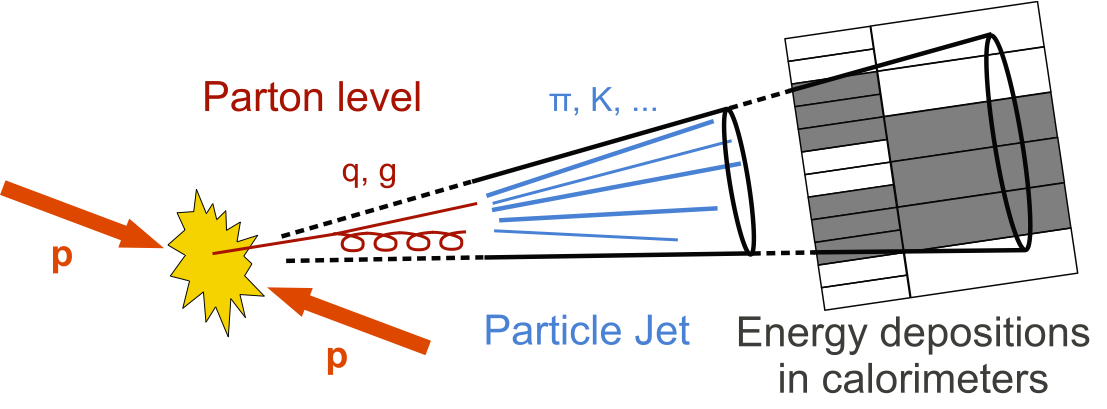
\includegraphics[width=.7\textwidth]{EventSelectionFigures/Sketch_PartonParticleCaloJet.png}
\caption{Sketch of pp-collision and resulting collimated spray of particles, a jet.}
\label{figs:jets}
\end{figure}  

As these jets of particles propagate through the CMS detector, they leave signals in components such as the tracker and the electromagnetic and hadronic calorimeters. These signals are combined using jet algorithms to form a reconstructed jet.  

\section{Event reconstruction}

Here events are reconstructed using the particle-flow reconstruction
algorithm~\cite{particleflow}, which attempts to reconstruct all
stable particles in an event by combining information from all
subdetectors. The algorithm categorizes all particles into five types:
muons, electrons, photons, charged and neutral hadrons. The resulting
particle flow candidates are passed to each jet clustering algorithm, in this case the
Cambridge-Aachen (CA)~\cite{CAaachen,CAcambridge}
jet clustering algorithm, as implemented in FastJet version 3.0.1 \cite{fastjet1,fastjet},
to create "particle flow jets".
The CA clustering sequence is only determined by the distance between
clusters and is not weighted by their momentum, as is done for the
$k_\text{T}$ and anti-$k_\text{T}$ algorithms. A distance parameter of
size $R=\sqrt{(\Delta \eta)^2 + (\Delta\phi)^2}=0.8$ is used for the CA algorithm.


Charged hadrons identified as pileup are removed from the inputs to
the jet clustering algorithms.  The remaining neutral component of pileup
is removed by applying a residual area-based correction as
described in Ref.~\cite{jetarea_fastjet,jetarea_fastjet_pu}.  The mean
$\pt$ per unit area is computed with the $k_{\mathrm T}$ algorithm
with the ``active area'' method, with a distance parameter of 0.6, and
the jet energy is corrected by the amount of pileup expected in the
jet area. The amount of energy expected from the underlying event is
added back into the jet.  The pileup-subtracted jet four momenta are
finally corrected for nonlinearities in $\eta$ and $\pt$ with
simulated data, with a residual $\eta$-dependent correction added to
correct for the difference in simulated and true
responses~\cite{JME-JINST,Collaboration:2012dp}.

\section{W, Z and H tagging}

\subsection{jet pruning}

As the mass of the V or H boson
is larger than the mass of a typical QCD jet, the jet mass is the
primary observable that distinguishes such a jet from a QCD jet.  The
bulk of the V or H jet mass arises from the kinematics of the two or
more jet cores that correspond to the decay quarks.  In contrast, the
QCD jet mass arises mostly from soft gluon radiation.  For this
reason, the use of jet pruning~\cite{jetpruning1,jetpruning2} improves
discrimination by removing the softer radiation, as this shifts the
jet mass of QCD jets to smaller values, while maintaining the jet mass
for V and H jets close to the masses of Z, W or H bosons.  Jet
pruning is implemented as additional cuts in the process of CA jet
clustering.  This algorithm starts from a set of ``protojets'' given
by the PF particles that form the original CA jet within a cone of
$R=0.8$.  These protojets are iteratively combined with each other
until a set of jets is found, however the large angle and low $\pt$
protojets are removed in the process.
The details of this procedure are given in~\cite{JME-13-006}.
%The distributions of pruned $\mathrm{m_j}$ for data, and for
The distributions of  the pruned jet mass ($\mathrm{m_j}$) for 
simulated signal and background samples, are shown in
Fig.~\ref{fig:JetMassTagging}.  Jets from boosted \PW\ and
\cPZ\ decays are expected to generate peaks at 
$\mathrm{m_j} \approx 80$ 
and $\mathrm{m_j} \approx$ 90 GeV, respectively. Jets
from boosted H decays are expected to peak at $\mathrm{m_j} \approx
120$ \GeVcc.
Hadronic top-quark jets, where the b quark and the
two different light quarks from the $\rm{t \to Wb \to q\bar{q'}b}$ decay are required
to be within a reconstructed jet of size R = 0.8, 
peak at $\mathrm{m_j} \approx 175$ \GeVcc.   
Jets from multijet events and not-fully-merged
W, \cPZ\ and H bosons give rise to a peak around 20\GeVcc, whose
size depends particularly on the spin and polarization of the boson.
All peaks are slightly shifted to lower masses, due to removal of soft
radiation by jet pruning.
If the pruned jet has a mass ($m_j$)
within 
$70 <m_j<100  \GeVcc $   
(  $110 < m_j <135 $ \GeVcc  ), 
% it is tagged as a $\PW/\cPZ$ ( H )
candidate. 


\begin{figure}[ht!b]
\begin{center}
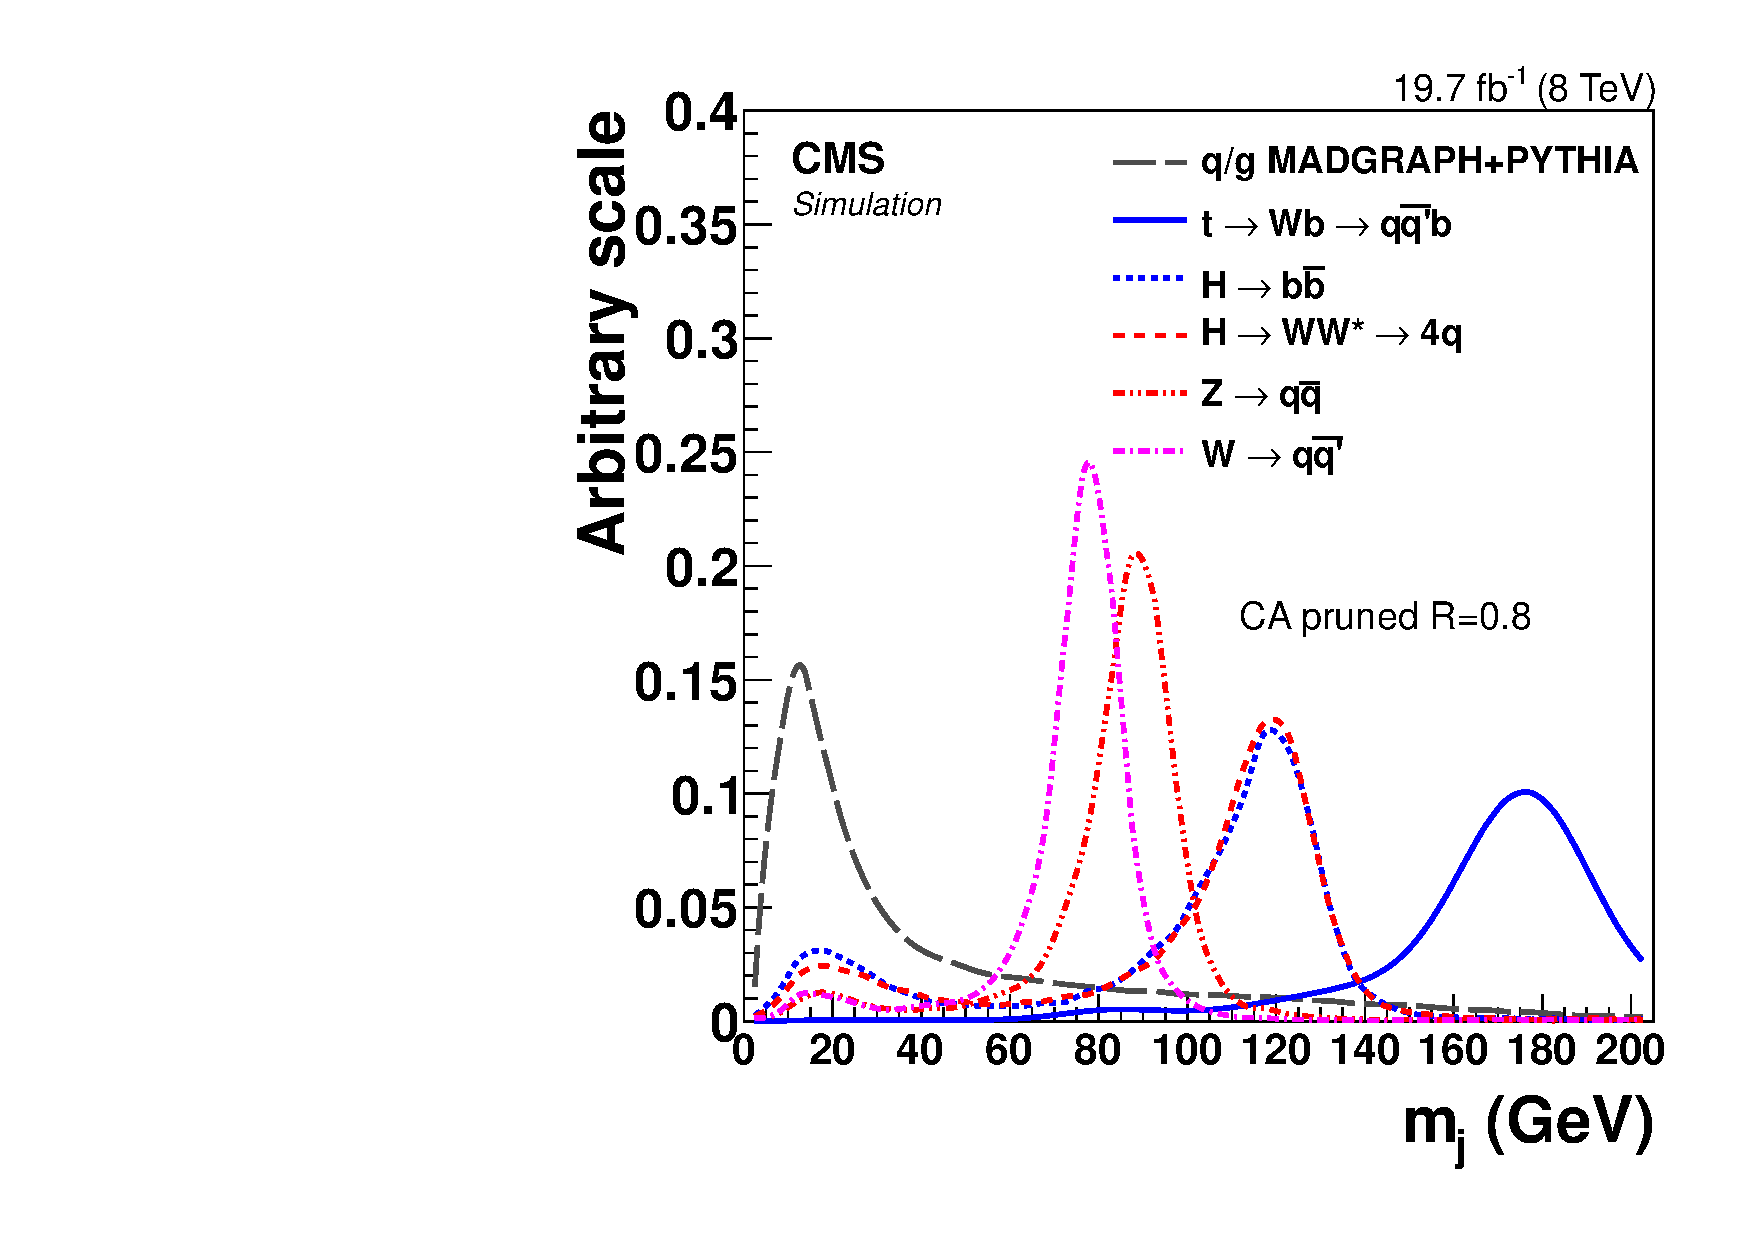
\includegraphics[width=0.69\textwidth]{EventSelectionFigures/signal-data-qcd-jetmass.pdf}
\end{center}
\caption{Distribution of pruned jet mass in
  simulation of signal and background processes.
  All simulated distributions are normalized to 1.
  The W/Z, H, and top-quark jets are required to
  match respective generator level particles in the event.
  The W/Z and H jets are from 1.5 TeV $\rm{W' \to WH}$ and 
  $\rm{Z' \to ZH}$ signal samples.
}  
\label{fig:JetMassTagging}
\end{figure}

\subsection{b tagging}
Jet pruning can also provide a good delineation of subjets within the CA8 jet.
%A dedicated b-tagging technique for boosted H tagging
% is used where the jet is split into two subjets, by reversing the last step of the CA8 pruning recombination algorithm. 
To tag jets from $\Hbb$ decays, denoted as ${\rm H_{bb}}$ jets, the pruned subjets, 
given by reversing the last step of the CA8 pruning recombination algorithm,  
are used as the basis for b tagging.
Jets arising from the hadronization of b quarks (b jets) are identified using the combined 
secondary vertex (CSV) b tagging algorithm~\cite{CSVBtagging}, which uses information from tracks and 
secondary vertices associated with jets to build a likelihood-based discriminator to distinguish
between jets from b quarks and those from charm or light quarks and gluons. The b tagging
discriminator can take values between 0 and 1 with higher values indicating higher probability
of the jet to originate from a b quark. 
The loose working point of the CSV algorithm~\cite{CSVBtagging} is chosen,
which is found to be optimal for both subjets and jets b tagging.  
It gives a b-tagging efficiency of $\approx$ 85\%,  
with mistagging probabilities of $\approx$ 40\% for 
c-quark jets and $\approx$ 10\% for light-quark and 
gluon jets with
 $\pt\approx 80\GeVcc$. The b-tagging efficiency ratio between data and
%simulation is applied as a scale factor~\cite{BTV-13-001} to 
the simulated signal events. To identify CA8 jets originating 
from H decays resulting in two collimated b jets, 
we apply b tagging 
either on the two subjets or the
CA8 jet, based on the angular separation of the
 two subjets ($\Delta $ R)~\cite{BTV-13-001}.
If $\Delta R$ between the CA8 subjets is bigger (smaller) than 0.3, 
b tagging is applied on both of the two subjets (on the CA8 jet). 




\subsection{N subjettiness}

We achieve additional discrimination against multijet events by
considering the distribution of jet constituents relative to the jet
axis. In particular, we quantify how well the constituents of a given
jet can be arranged into $N$ subjets. This is done by reconstructing
the full set of jet constituents (before pruning) with the \kt
algorithm~\cite{ktalg} and halting the reclustering when $N$
distinguishable protojets are formed.  
The directions of the $N$ jets are used as the reference axes to
compute the
$N$-subjettiness~\cite{Thaler:2010tr,Thaler:2011gf,Stewart:2010tn}
$\tau_{N}$ of the original jet, defined as
\begin{equation}
\label{eq:subjettiness}
%\tau_N = \frac{1}{d_{0}} \sum_{k} \ptk\,\min( \Delta R_{1,k}, \Delta R_{2,k},\ldots,\Delta R_{N,k}),
\tau_N = \frac{1}{d_{0}} \sum_{k} \ptk\,\min( \Delta R_{1,k}, \Delta R_{2,k},\ldots,\Delta R_{N,k}),
\end{equation}
%
where $\ptk$ is the $\pt$ of the particle constituent $k$ of the
original jet, and $\Delta R_{n,k}$ is its angular distance from the
axis of the $n$th subjet (with $n=1, 2,\ldots,N$). The normalization
factor $d_{0}$ for $\tau_N$ is $d_{0}= \sum_{k} \ptk R_{0}$, with
$R_{0}$ set to the distance parameter $R$ of the original CA jet. To
improve the discriminating power, we perform a one-pass optimization
of the directions of the subjet axes by minimizing
$\tau_{N}$~\cite{Thaler:2011gf,JME-13-006}.  By using the smallest
$\Delta R_{n,k}$ to weight the value of $\ptk$ in
Eq.~(\ref{eq:subjettiness}), $\tau_N$ yields small values when the jet
originates from the hadronization of $N$ quarks. 
The $\tau_{ij} = \tau_{i} / \tau_{j}$
ratios $\tau_{21}$, $\tau_{31}$, 
$\tau_{32}$, $\tau_{41}$, $\tau_{42}$, and $\tau_{43}$ 
have been studied to identify
the best discriminators for jets from $\Hww$ and $\Vqq$ decays. 
%We find that the ratio $\tau_{42}=\tau_{4} / \tau_{2}$
We find that the ratio $\tau_{42}$
works best to discriminate the four-pronged $\Hww$ events against QCD jets,
 and $\tau_{21}$
to identify $\Vqq$~\cite{Khachatryan:2014hpa}.
The discriminating power of $\tau_{21}$  and $\tau_{42}$ for
different resonance models can be seen in
Fig.~\ref{fig:taggingvariables} and Fig.~\ref{fig:tau422TeV}, respectively. 



\begin{figure}[th!b]
\centering
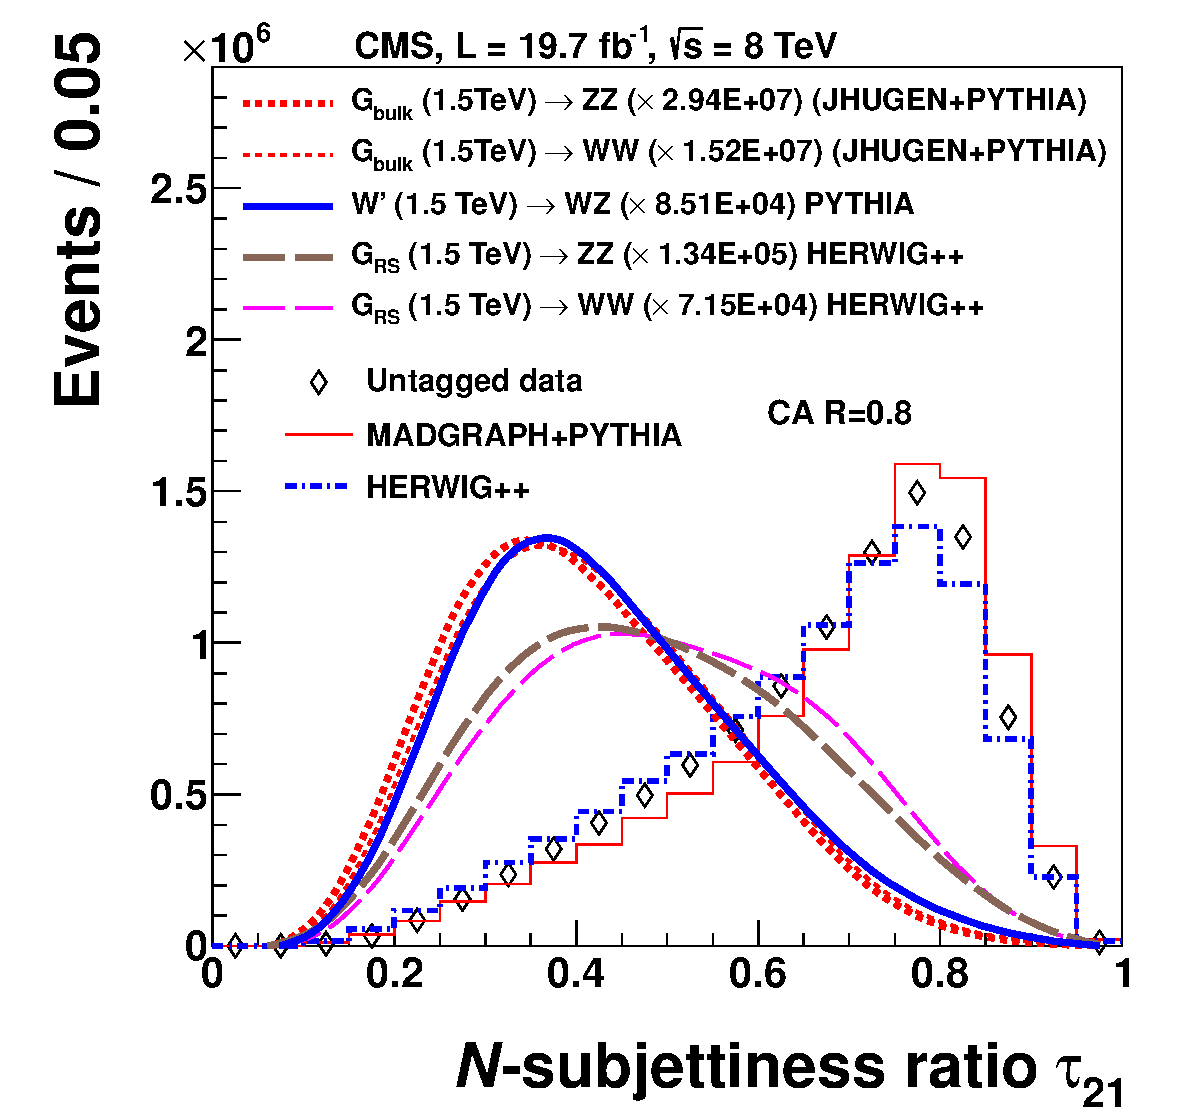
\includegraphics[width=0.49\textwidth]{EventSelectionFigures/signal-data-qcd-Jet-Tau21.pdf}
  \caption{Distribution for jet
   $N$-subjettiness ratio $\tau_{21}$ in data, and in simulations
   of signal and background events. All simulated distributions are
   scaled to match the number of events in data. \MADGRAPH/\PYTHIA and
   \HERWIG{++} refer to QCD multijet event
   simulations.\label{fig:taggingvariables}}
\end{figure}

\begin{figure}[ht!b]
\centering
\begin{tabular}{cc}
     \resizebox{0.5\linewidth}{!}{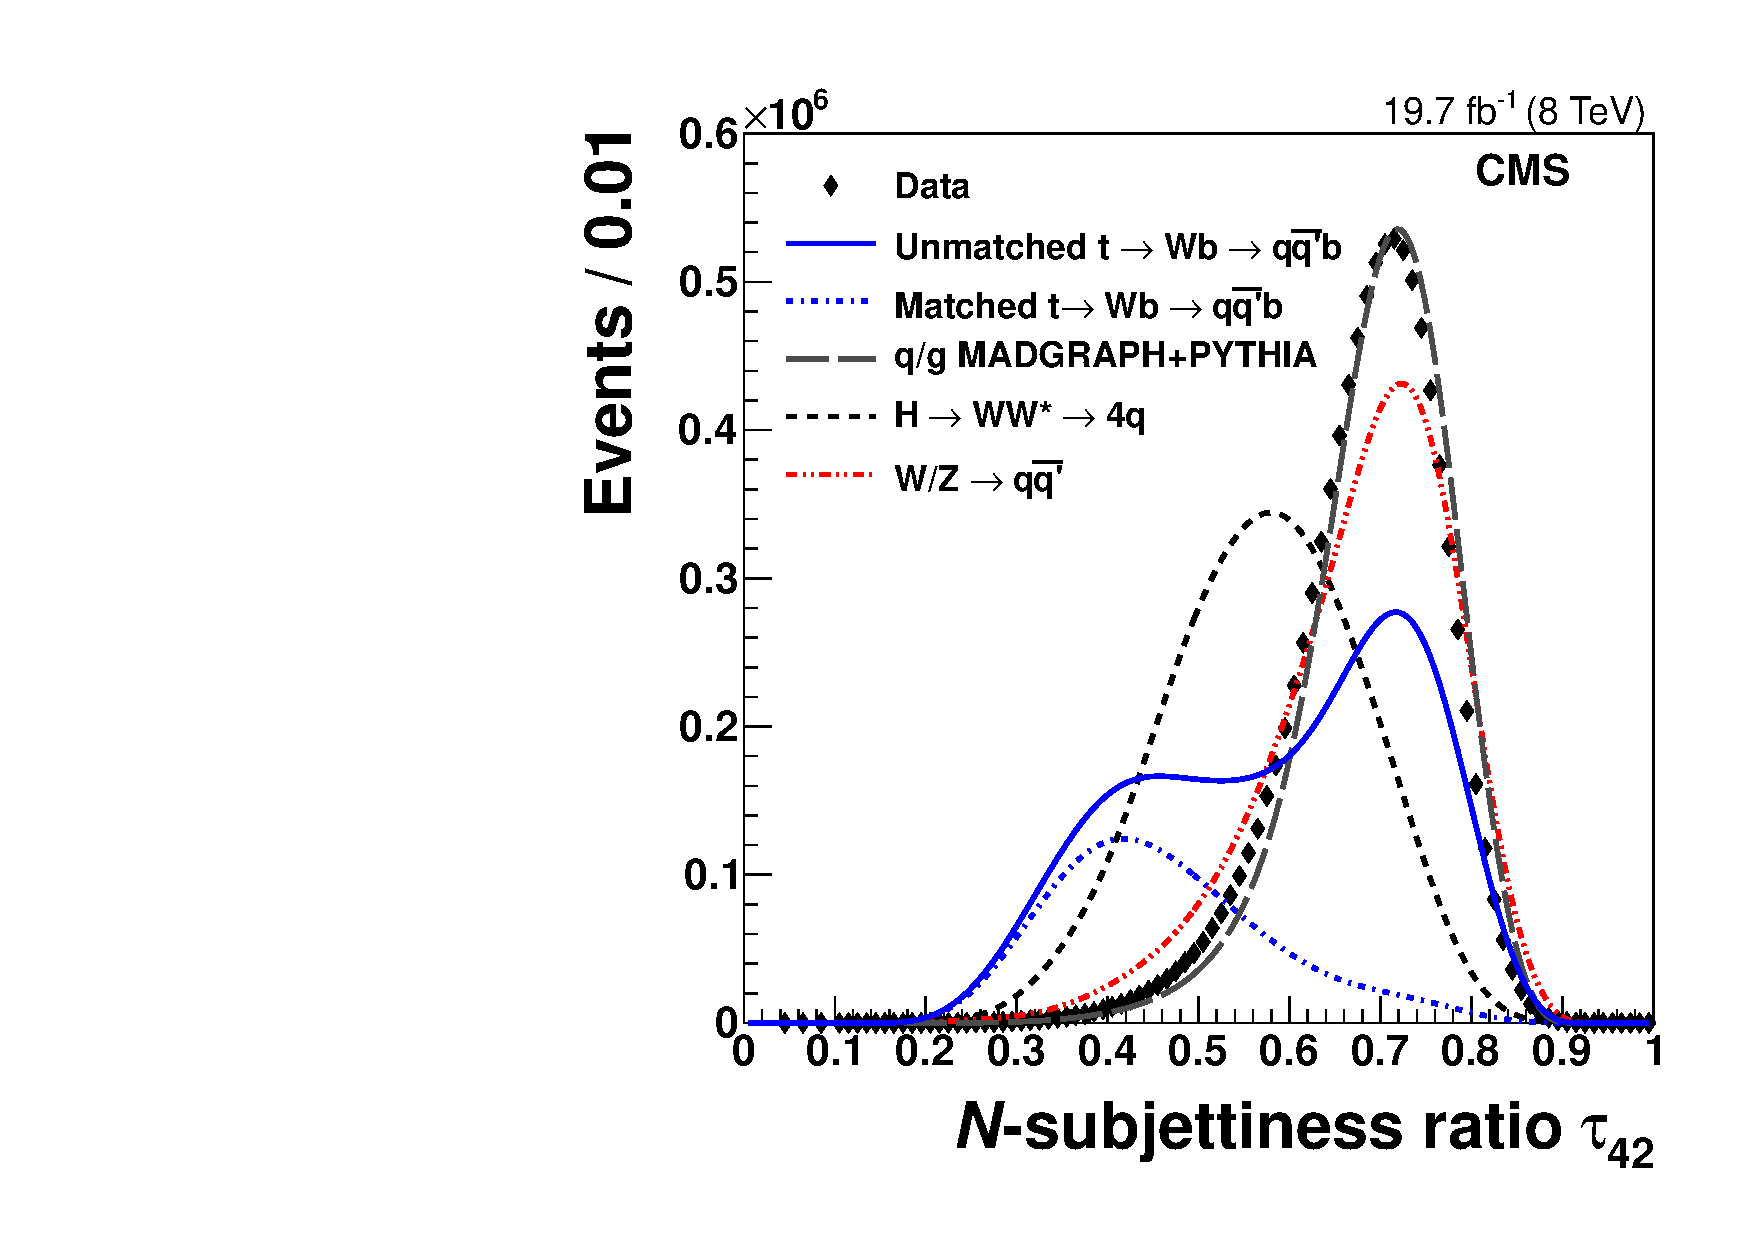
\includegraphics{EventSelectionFigures/tau42PlotAllPre.pdf}} &
     \resizebox{0.5\linewidth}{!}{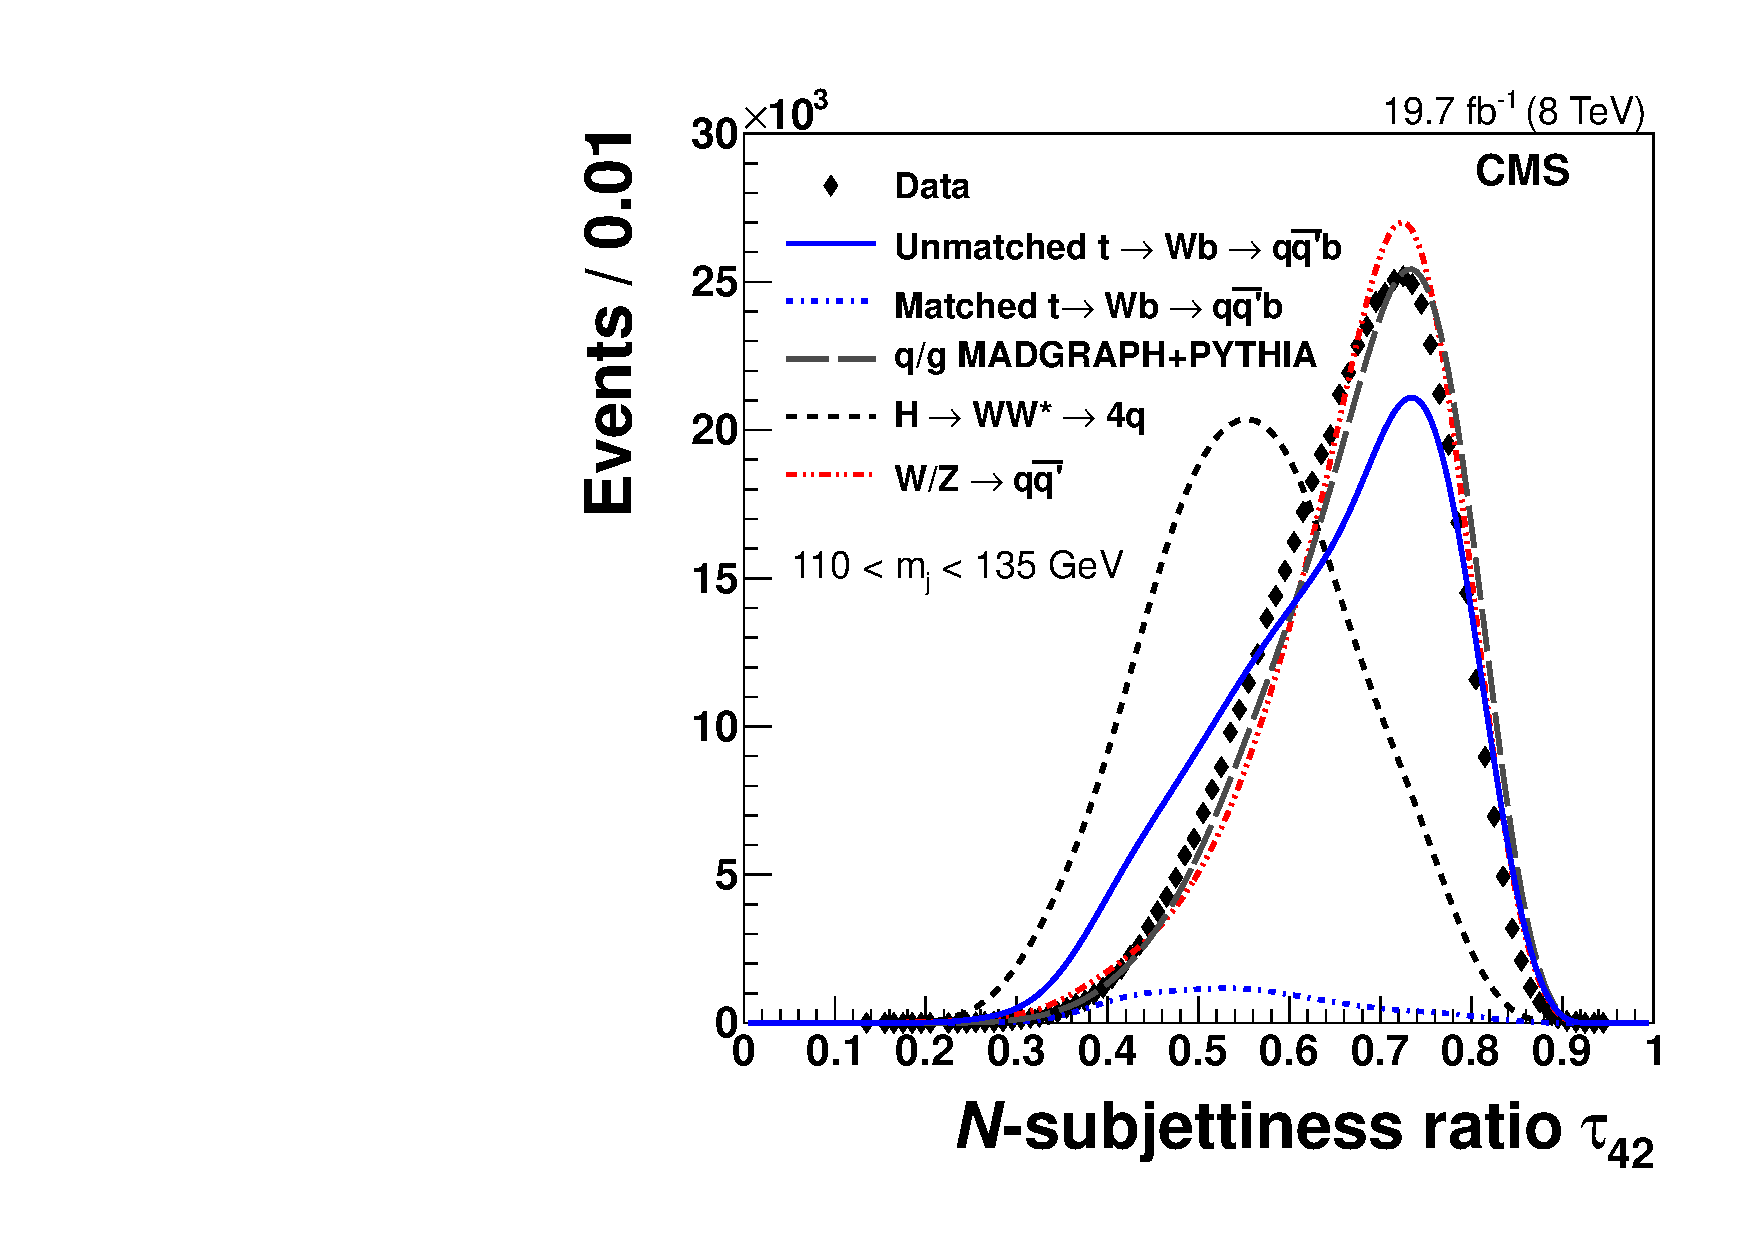
\includegraphics{EventSelectionFigures/tau42PlotAllAfter.pdf}} \\
\end{tabular}
\caption
{
  Distributions of $\tau_{42}$ in
  data and in simulations of signal (2 TeV) and background events, without applying 
  the pruned jet mass requirement (left) 
  and with the pruned jet mass requirement applied (right). 
  W/Z, matched top-quark, and ${\rm H_{WW}}$ jets are required to
  match their generator level particles, respectively.
  All simulated distributions are scaled to match the number
  of events in data, except that matched top-quark background is scaled to 
  the fraction of unmatched ${\rm t\bar{t}}$ events times
  the number of data events.
  } 
\label{fig:tau422TeV}
\end{figure}
























